E' richiesto un set di immagini con le seguenti specifiche: 
\begin{itemize}
    \item 8 Immagini di dimensione $512 \times 512$;
    \item Formato PNG in scala dei grigi;
    \item Devono contenere tra i 2 ed i 6 oggetti geometrici;
    \item Oggetti di colore uniforme su uno sfondo nero.
\end{itemize}


Useremo anche altre due immagini di tipo fotografico/medico/astronomico a scelta trovate su internet.
Quest'ultime saranno importate all'interno del progetto con la libreria \code{skimage}, impostando il flag \verb|as_gray=True| per averle in bianco e nero.

Le immagini selezionate sono le seguenti:
\begin{description}
    \item[Immagine Con Testo] Composizione di prime pagine di giornale con i relativi articoli.
    \item[Immagine Fotografica] Che ritrae il volto di una persona in modo dettagliato e con varie tonalità di grigio.
\end{description}

\begin{figure}
    \centering
    \subfigure
    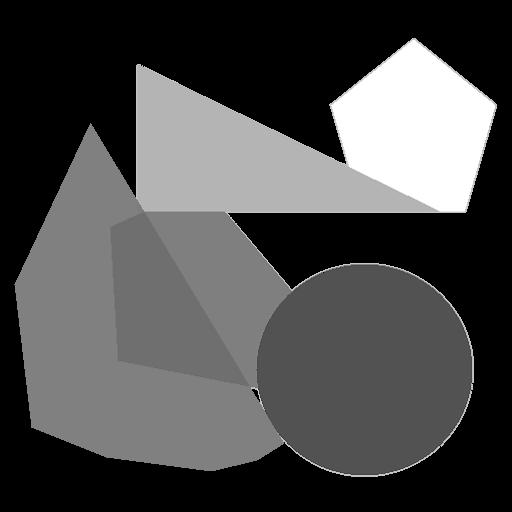
\includegraphics[width=5cm]{img1}\hfil
    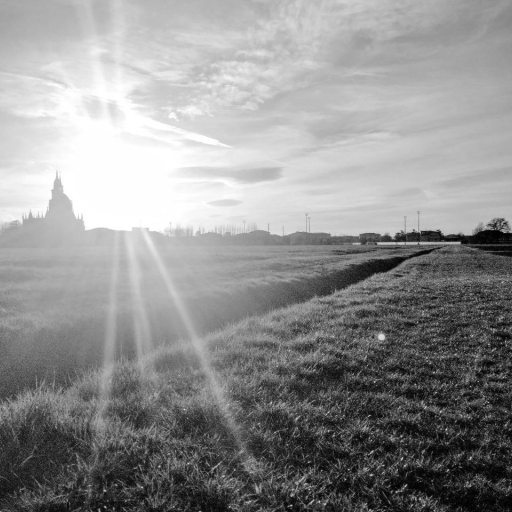
\includegraphics[width=5cm]{paesaggio}
    \caption{Immagine geometrica originale img1.png}
    \label{fig:img1}
    \caption{Immagine fotografica originale paesaggio.png}
    \label{fig:paesaggio}
\end{figure}
